\chapter{Tekstverwerking}

\section{Tekens en tekenreeksen}Veel computerprogramma's moeten tekstuele informatie kunnen vastleggen in de vorm van afdrukbare letters, cijfers en symbolen. De behoefte aan tekst ontstaat bij tekstverwerkingsprogramma's en woordspellen. Ook bij natuurlijke taalverwerking en bij tekstgebaseerde avonturenspellen is tekst nodig, omdat beide de invoer moeten begrijpen. Het begrijpen van tekstinvoer heet {\it parsen}. Kortom, tekstverwerking wordt overal toegepast. Om dergelijke informatie in te voeren, weer te geven en te bewerken, moeten wij twee kernbegrippen introduceren: tekens en tekenreeksen.

Tekens kunnen afdrukbaar of niet-afdrukbaar zijn. Een teken vertegenwoordigt meestal één enkel, primitief element van afdrukbare tekst, dat met de {\bf PRINT}-opdracht op het scherm kan worden weergegeven. Het meest voor de hand liggend en natuurlijk is het om een teken op te vatten als een letter uit een alfabet. Een teken kan bijvoorbeeld een van de hoofdletters 'A' tot 'Z' zijn, of een van de kleine letters 'a' tot 'z'. Tekens kunnen echter ook veelgebruikte symbolen vertegenwoordigen, zoals leestekens of valutasymbolen. Zij kunnen zelfs de decimale cijfers '0' tot '9' vertegenwoordigen. Het is goed om te beseffen dat het hier om de tekstuele weergave van de cijfers 0 tot 9 als afdrukbare symbolen gaat en niet om hun numerieke tegenhangers. Daarnaast biedt de MEGA65 een uitgebreide reeks speciale symbolen die samen kunnen worden gebruikt voor spellen, voor het tekenen van sierlijke randen of kunst. Naast het weergeven van informatie kunnen zulke symbolen ook eenvoudige, doch boeiende visuele patronen vormen. Voor het gemak staan deze speciale symbolen op de voorzijde van de toetsen van de MEGA65.

Een teken kan ook niet-afdrukbaar zijn. Het gebruik van dergelijke tekens (in een {\bf PRINT}-opdracht) kan bepaald gedrag activeren of bepaalde modi actief maken, zoals het omzetten van alle tekst op het scherm naar kleine letters of het instellen van de voorgrondkleur op oranje. Andere niet-afdrukbare tekens kunnen een regelterugloop vertegenwoordigen of het scherm wissen.

Voor een volledig overzicht van de beschikbare tekens verwijzen wij u naar \bookvref{appendix:petsciicodes}. De tabel vermeldt de tekens die bij een bepaald codenummer horen. Het codenummer moet als argument aan de {\bf CHR\$}-functie worden meegegeven; in combinatie met de {\bf PRINT}-opdracht geeft dat de bijbehorende tekens op het scherm weer.

Hier ziet u een voorbeeld van het weergeven van het uitroepteken met behulp van een tekencode:

\begin{screencode}
PRINT CHR$(33)
!
\end{screencode}

Merk op dat het '!'-teken inderdaad op het scherm zichtbaar is, omdat het een afdrukbaar teken is.

Hier ziet u een voorbeeld van het veranderen van de voorgrondkleur naar wit met behulp van tekencodes:

\begin{screencode}
PRINT CHR$(5)
\end{screencode}

Hoewel er geen teken wordt weergegeven, krijgen alle afdrukbare tekens die daarna op het scherm verschijnen de kleur wit.

Soms is het nuttig om de omzetting omgekeerd uit te voeren: van een teken naar het bijbehorende codenummer. Hiertoe moet één enkel teken, tussen aanhalingstekens, als argument aan de {\bf ASC}-functie worden meegegeven; in combinatie met de {\bf PRINT}-opdracht geeft dat het bijbehorende codenummer decimaal op het scherm weer.

Hier ziet u een voorbeeld van het bepalen van het codenummer van het uitroepteken.

\begin{screencode}
PRINT ASC("!")
 33
\end{screencode}

En hier ziet u een voorbeeld van het bepalen van het codenummer van het uitroepteken en het opslaan ervan in een integer-variabele:
\begin{screencode}
A% = ASC("!")
\end{screencode}

Hoewel we afzonderlijke tekens herhaaldelijk kunnen weergeven met {\bf CHR\$}, zou het omslachtig zijn om dit steeds op deze manier te doen.

Het begrip tekenreeks is nodig, omdat het het idee van een aaneengesloten blok tekst vertegenwoordigt. Een tekenreeks kan dus meerdere afdrukbare en/of meerdere niet-afdrukbare tekens bevatten, in elke gewenste combinatie. Een tekenreeks kan ook leeg zijn en helemaal geen tekens bevatten. Om een tekenreeks te schrijven, zetten we het teken\(s\) tussen aanhalingstekens. De reeks "HALLO WERELD!" is bijvoorbeeld een tekenreeksconstante.

\begin{screencode}
PRINT "HALLO WERELD!"
HALLO WERELD!
\end{screencode}

Alle tekenreeksen hebben een eigenschap met de naam lengte, welke aangeeft hoeveel afdrukbare en niet-afdrukbare tekens er in die tekenreeks aanwezig zijn. De lengte kan variëren van 0 (de lege tekenreeks) tot 255. Een poging om een tekenreeks te maken die langer is dan 255 tekens, leidt tot een {\bf ?STRING TOO LONG ERROR}.

\begin{screencode}
PRINT LEN("HALLO WERLED!")
 12
\end{screencode}

\begin{screencode}
PRINT LEN("")
 0
\end{screencode}

Het is mogelijk om variabelen te maken die specifiek voor tekenreeksen bedoeld zijn. Alle dergelijke tekenreeksvariabelen hebben namen die met een letter beginnen, eventueel een tweede, alfanumeriek teken bevatten en op een \$ eindigen. Nadat zij een waarde hebben gekregen, kunnen zij met {\bf PRINT} worden gebruikt.

\begin{screencode}
AB$ = "HALLO WERELD!": PRINT AB$
HALLO WORLD!
\end{screencode}

\begin{screencode}
A1$ = "HALLO WERELD!": PRINT LEN(A1$)
 12
\end{screencode}

\section{Tekenreeksconstanten}Tekenreeksconstanten kunnen met één of meer andere tekenreeksconstanten worden samengevoegd tot een samengestelde tekenreeks. Dit proces heet {\it samenvoegen}. Om twee of meer tekenreeksconstanten samen te voegen, koppelt u ze met de +-operator aan elkaar.

Hier volgen enkele voorbeelden:

\begin{screencode}
PRINT ("TWEEDE" + "HANDS")
TWEEDEHANDS
\end{screencode}

\begin{screencode}
PRINT ("AUTOBAND" + "VENTIEL" + "DOPJE")
AUTOBANDVENTIELDOPJE
\end{screencode}

Soms zijn leestekens of spaties nodig om de uiteindelijke uitvoer er correct opgemaakt te laten uitzien, zoals in het volgende voorbeeld.

\begin{screencode}
PRINT ("FRUIT: " + "APPEL, " + "PEER EN " + "FRAMBOOS.")
FRUIT: APPEL, PEER EN FRAMBOOS.
\end{screencode}

\section{Tekenreeksvariabelen}

Samenvoegen komt vaker voor bij tekenreeksvariabelen in combinatie met tekenreeksconstanten. In een tekstgebaseerd avonturenspel wilt u bijvoorbeeld enkele uitgangen vermelden, zoals noord of zuid. Omdat deze uitgangen afhankelijk zijn van de plek waar u zich op dat moment bevindt, is het zinvol om variabelen voor de uitgangen zelf te gebruiken en om de uitvoer met constanten, zoals komma's, spaties en punten, passend op te maken.

\begin{screencode}
A$ = "PINDA": B$ = "KAAS": PRINT (A$ + B$ + "POT")
PINDAKAASPOT
\end{screencode}

Het is ook mogelijk om tekenreeksen als parameters van {\bf DATA}-opdrachten te gebruiken, zodat zij later met het {\bf READ}-opdrachten kunnen worden ingelezen. Het volgende voorbeeld laat tevens zien dat arrays ook tekenreeksen kunnen bevatten.

\begin{screencode}
10 DIM A$(6)
20 PRINT "KLEUREN VAN DE REGENBOOG: ";
30 FOR I = 0 TO 5
40 :  READ A$(I): PRINT (A$(I) + ", ");
50 NEXT I
60 READ A$(I): PRINT ("AND " + A$(I) + ".")
70 DATA "ROOD", "ORANJE", "GEEL", "GROEN", "BLAUW", "INDIGO", "VIOLET"
\end{screencode}

Het komt vaak voor dat tekenreeksgegevens of gegevens van één enkel teken rechtstreeks uit gebruikersinvoer afkomstig zijn. Wanneer de gebruiker tekst intoetst, zal die tekst vaak geparst moeten worden of terug naar het scherm moeten worden weergegeven. In het algemeen zijn er drie hoofdmanieren om dat te doen: via de {\bf GET}-opdracht, via de {\bf GETKEY}-opdracht of via de {\bf INPUT}-opdracht.

Alle drie de opdrachten gedragen zich verschillend. Het is daarom belangrijk om ze met elkaar te vergelijken en tegen elkaar af te zetten, zodat u begrijpt hoe elk ervan werkt.

De {\bf GET}-opdrachten is handig om de huidige toetsaanslag in een variabele op te slaan. Het programma wacht niet op een toetsaanslag: het gaat onmiddellijk door met het uitvoeren van de volgende opdracht. Om die reden is het soms belangrijk om de {\bf GET}-opdracht binnen een of andere lus te plaatsen---de lus wordt pas verlaten wanneer een geldige toetsaanslag is gedetecteerd. Als de variabele die aan {\bf GET} wordt meegegeven een tekenreeksvariabele is en er geen toetsaanslag wordt gedetecteerd, dan krijgt die tekenreeksvariabele de waarde van een lege tekenreeks.

\begin{screencode}
10 GET A$: REM WACHT NIET OP EEN TOETSDRUK--LEES EEN TOETSDRUK IN DE VARIABELE
20 PRINT A$: IF (A$ = "J" OR A$ = "N") THEN END
30 GOTO 10
\end{screencode}

De {\bf GETKEY}-opdracht is ook nuttig om de huidige toetsaanslag in een variabele op te slaan. In tegenstelling tot de {\bf GET}-opdracht wacht de {\bf GETKEY}-opdracht bij de uitvoering wel degelijk op één toetsaanslag voordat het doorgaat met het uitvoeren van de volgende opdracht.

\begin{screencode}
10 GETKEY A$: WACHT OP EEN TOETSDRUK--PAUZEER EN LEES 'M IN DE VARIABELE
20 PRINT A$: IF (A$ = "J" OR A$ = "N") THEN END
30 GOTO 10
\end{screencode}

Waar {\bf GET} en {\bf GETKEY} goed geschikt zijn voor het lezen van losse tekens, is de {\bf INPUT}-opdracht nuttig voor het inlezen van complete tekenreeksen---dat wil zeggen, nul of meer tekens per keer.

Wanneer de {\bf INPUT}-opdracht met een komma en een variabele wordt gebruikt, verschijnt de prompttekst op de gewone manier, met een cursor waarmee de gebruiker tekst kan intypen. Wanneer de {\bf INPUT}-opdracht met een puntkomma en een variabele wordt gebruikt, verschijnt de prompttekst met een toegevoegd vraagteken en met een cursor waarmee de gebruiker tekst kan intypen.

\begin{screencode}
10 INPUT "VOER UW NAAM IN", A$: REM GEEN VRAAG
20 PRINT ("HALLO " + A$)
\end{screencode}

\begin{screencode}
10 INPUT "HOE HEET U"; A$: REM VRAAG
20 PRINT ("HALLO " + A$)
\end{screencode}

In beide gevallen rondt het indrukken van \specialkey{RETURN} de tekstinvoer af---de ingevoerde tekst wordt in de opgegeven variabele opgeslagen. Merk op dat wanneer de tekenreeksvariabele al een tekenreeks bevat en \specialkey{RETURN} wordt ingedrukt zonder dat er nieuwe gegevens worden ingetypt, de oude tekenreekswaarde die zich momenteel in de variabele bevindt, behouden blijft.

\section{Tekenreeksfuncties}Er zijn drie veelgebruikte functies voor het bewerken van tekenreeksen: {\bf MID\$}, {\bf LEFT\$} en {\bf RIGHT\$}. Deze zijn bij uitstek geschikt voor het isoleren van deelreeksen, waaronder afzonderlijke tekens.

Het volgende programma vraagt om een invoertekenreeks en geeft daarna alle linkerdeelreeksen weer.
\begin{screencode}
10 INPUT "VOER EEN WOORD IN:", A$
20 PRINT "ALLE LINKER DEELTEKENREEKSEN ZIJN:"
30 FOR I = 0 TO LEN(A$)
40 :  PRINT LEFT$(A$, I)
50 NEXT I
\end{screencode}

Het volgende programma vraagt om een invoertekenreeks en geeft daarna alle rechterdeelreeksen weer.
\begin{screencode}
10 INPUT "VOER EEN WOORD IN:", A$
20 PRINT "ALLE RECHTER DEELTEKENREEKSEN ZIJN:"
30 FOR I = 0 TO LEN(A$)
40 :  PRINT RIGHT$(A$, I)
50 NEXT I
\end{screencode}

Het volgende programma vraagt om een invoertekenreeks die bestaat uit een voornaam, gevolgd door een spatie en daarna een achternaam. Het geeft vervolgens de beginletters van beide namen weer.
\begin{screencode}
10 INPUT "VOOR EEN VOORNAAM, EEN SPATIE EN EEN ACHTERNAAM IN:", A$
20 N = -1
30 FOR I = 1 TO LEN(A$)
40 :  IF (MID$(A$, I, 1) = " ") THEN N = I: GOTO 60
50 NEXT I
60 IF (N = -1) THEN GOTO 10
70 PRINT "INITIALEN ZIJN: "; MID$(A$, 1, 1)+"."+MID$(A$, N + 1, 1)+"."
\end{screencode}

\section{Eenvoudige opmaak}

\subsection{Nieuwe regels onderdrukken}Wanneer de {\bf PRINT}-opdracht in een programma wordt gebruikt, is het standaardgedrag dat de tekenreeks wordt weergegeven en dat de cursor daarna naar de volgende regel gaat. Om te voorkomen dat de cursor automatisch naar de volgende regel gaat, plaatst u eenvoudigweg een ; (puntkomma) achter het einde van de tekenreeks. Vergelijk de regels 10, 20 en 30 in het volgende programma.

\begin{screencode}
10 PRINT "DIT IS EEN ENKELE REGEL TEKST": REM ER WORDT EEN NIEUWE REGEL BEGONNEN
20 PRINT "THE SECOND LINE"; : REM EEN NIEUWE REGEL WORDT ONDERDRUKT
30 PRINT " USES A SEMICOLON" : REM EEN REGEL WORDT AAN DE VORIGE VASTGEMAAKT
\end{screencode}

\subsection{Automatische tabstops}Soms is het handig om de {\bf PRINT}-opdracht te gebruiken om informatie netjes in kolommen weer te geven. Dit kunt u doen door een , (komma) achter het einde van de tekenreeks te plaatsen. Bekijk het volgende voorbeeldprogramma.

\begin{screencode}
10 PRINT "TEKST 1", "TEKST 2", "TEKST 3", "TEKST 4"
\end{screencode}

Merk op dat de tabstops telkens 10 tekens uit elkaar liggen. TEKST 1 begint dus in kolom 0, TEKST 2 begint in kolom 10, TEKST 3 begint in kolom 20 en TEKST 4 begint in kolom 30.

\subsection{Tabstops en spatiëring}Bij het weergeven van tekst op het scherm is het vaak nodig om tekst op te maken met behulp van spaties en tabs. Twee commando's zijn hierbij behulpzaam: {\bf SPC} en {\bf TAB}.

Het commando {\bf SPC(5)} schuift bijvoorbeeld vijf tekens naar rechts. Alle tekens die zich tussen de huidige cursorpositie en de positie vijf tekens verder naar rechts bevinden, blijven onveranderd staan.

Het commando {\bf TAB(20)} gaat bijvoorbeeld naar kolom 20 door de huidige cursorpositie van twintig af te trekken en vervolgens dat aantal tekens naar rechts te schuiven. Ligt de beginpositie van de cursor rechts van kolom 20, dan doet het commando niets. Dit commando is vaak bruikbaar om tekst netjes in kolommen uit te lijnen.

\section{Voorbeeldprogramma's}

We sluiten af met enkele voorbeelden.

\subsection{Palindromen}

Een {\it palindroom} is een woord, zin of getal dat voorwaarts en achterwaarts gelezen hetzelfde is. Enkele voorbeelden zijn: CIVIC, LEVEL, RADAR, MADAM en 1234321. Het volgende programma draait de ingevoerde tekst om en bepaalt vervolgens of de oorspronkelijke zin gelijk is aan de omgekeerde zin.

% \begin{screencode}
\begin{tcolorbox}[colback=black,coltext=white]
\verbatimfont{\codefont}
\begin{verbatim}
10 REM *** PALINDROMEN ***
20 INPUT "VOER WAT TEKST IN: ", A$
30 B$ = ""
40 FOR I = 1 TO LEN(A$)
50 :  B$ = MID$(A$, I, 1) + B$
60 NEXT I
70 IF (A$ = B$) THEN PRINT (A$ + " IS EEN PALINDROOM"): ELSE PRINT (A$ + " IS GEEN PALINDROOM")
80 GOTO 20
\end{verbatim}
\end{tcolorbox}
% \end{screencode}


\subsection{Eenvoudige cijfers}

Nu bekijken we drie eenvoudige voorbeelden van het versleutelen en ontsleutelen van Engelstalige tekstberichten. Dit proces van versleutelen en ontsleutelen is het studiegebied van de {\it cryptografie} en wordt toegepast om informatie beveiligd te houden, zodat anderen deze niet kunnen lezen, behalve wie het voorrecht heeft de methode en de geheime sleutel van het cijfer te kennen.

Het proces waarbij een gegeven bericht wordt versleuteld, heet {\it encryptie}. De gewone, leesbare, onversleutelde tekst heet {\it klare tekst}. Het versleutelen van klare tekst levert een door elkaar gehaald bericht op; deze versleutelde tekst heet {\it cijfertekst}. Het proces waarbij de cijfertekst wordt ontsleuteld, heet {\it decryptie}. Het ontsleutelen van de cijfertekst levert weer een leesbaar bericht op --- de klare tekst.

Stel dat wij een stuk klare tekst versleutelen en de resulterende cijfertekst vervolgens naar een vriend sturen. Indien die vriend de methode en de geheime sleutel kent die voor het versleutelen van het bericht zijn gebruikt, kan deze de cijfertekst ontsleutelen en zo ons oorspronkelijke bericht in klare tekst herstellen en lezen.

Als iemand anders probeert de cijfertekst te lezen met de verkeerde methode en/of de verkeerde geheime sleutel, is de resulterende tekst onbegrijpelijk.

De cryptografische systemen die we hier beschrijven, zijn zeer eenvoudig. Uiteraard zou men ze tegenwoordig niet meer moeten gebruiken, omdat cryptanalysetechnieken ze gemakkelijk kunnen kraken. Ze illustreren echter wel enkele basistechnieken en laten zien hoe we een voorbeeldprogramma kunnen opbouwen.

We bekijken drie cijfers: het ROT13-cijfer, het Caesar-cijfer en het Atbasj-cijfer. Deze maken deel uit van een groep cijfers die bekend staat als {\it affiene cijfers}.

Wiskundig gezien is het nuttig om de letters van het Nederlandse alfabet als genummerd te beschouwen. A is 0, B is 1 enzovoort, waarbij Z gelijk is aan 25.

\begin{center}
{\setlength{\tabcolsep}{0.74mm}
\ttfamily

  \begin{tabular}{|c|c|c|c|c|c|c|c|c|c|c|c|c|c|c|c|c|c|c|c|c|c|c|c|c|c|c|}
  \hline
     Letter & A & B & C & D & E & F & G & H & I & J & K & L & M & N & O & P & Q & R & S & T & U & V & W & X & Y & Z \\ \hline	Waarde & 0 & 1 & 2 & 3 & 4 & 5 & 6 & 7 & 8 & 9 & 10 & 11 & 12 & 13 & 14 & 15 & 16 & 17 & 18 & 19 & 20 & 21 & 22 & 23 & 24 & 25 \\ \hline
  \end{tabular}
}
\end{center}

Een belangrijk wiskundig onderdeel van een cryptografisch systeem is {\it modulair rekenen}, soms informeel ``rekenen met een klok'' genoemd, omdat de getallen bij nul beginnen en oplopen tot een bovengrens, waarna ze weer naar nul teruggaan, net als bij een cirkel. In ons geval, aangezien het Nederlandse alfabet 26 letters telt, rekenen we modulo 26---onze letters zijn genummerd van 0 tot 25.
\begin{center}
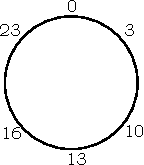
\includegraphics{images/illustrations/modular.pdf}
\end{center}

Om een gegeven getal modulo 26 te herleiden, kunnen we de volgende functie gebruiken:

\[
 f(x) = x - \left\lfloor{\frac{x}{26}}\right\rfloor \times 26
\]

Hieruit blijkt dat we, om de waarde van een getal $x$ modulo 26 te verkrijgen, eerst $x$ door 26 delen en naar beneden afronden, waarmee we het aantal keren bepalen dat we de cirkel rond zijn gegaan. Daarna vermenigvuldigen we dit resultaat weer met 26 en trekken we het van $x$ af. Het eindresultaat is de rest die overblijft en zal altijd een waarde tussen 0 en 25 zijn.

Als voorbeeld is het getal 28 in modulo 26 gelijk aan 2:
\[
	f(28) = 28 - \left\lfloor{\frac{28}{26}}\right\rfloor \times 26 = 28 - 1 \times 26 = 2
\]

Het programma aan het einde van dit hoofdstuk gebruikt deze formule door op regel 30 een overeenkomstige functie te definiëren:

\begin{screencode}
DEF FN F(X)=X-INT(X/26)*26
\end{screencode}

{\bf ROT13:} Om elke letter uit de klare tekst te versleutelen, schuiven we 13 plaatsen naar voren. De letter A uit de klare tekst wordt zo de letter N uit de cijfertekst, B wordt O, waarbij de laatste letters ``terugspringen'' naar het begin van het alfabet. De letter Z uit de klare tekst wordt daardoor de letter M uit de cijfertekst. Hiermee is de versleuteling beschreven. Het ontsleutelen van de cijfertekst werkt op precies dezelfde manier: we herhalen het proces eenvoudigweg door opnieuw 13 plaatsen naar voren te schuiven, waardoor de cirkel rond is en we weer uitkomen waar we begonnen. Zo wordt de letter N uit de cijfertekst weer de letter A uit de klare tekst.

We kunnen dit visueel zien als een afbeelding in tabelvorm:

\Large
\begin{center}
  \begin{tabular}{|c|c|c|c|c|c|c|c|c|c|c|c|c|c|}
  \hline
    Klare tekst & A & B & C & D & E & F & G & H & I & J & K & L & M \\ \hline	ROT13-cijfertekst & N & O & P & Q & R & S & T & U & V & W & X & Y & Z \\ \hline
  \end{tabular}
\end{center}

\begin{center}
  \begin{tabular}{|c|c|c|c|c|c|c|c|c|c|c|c|c|c|}
  \hline
    Klare tekst & N & O & P & Q & R & S & T & U & V & W & X & Y & Z \\ \hline	ROT13-cijfertekst & A & B & C & D & E & F & G & H & I & J & K & L & M \\ \hline
  \end{tabular}
\end{center}

\normalsize

Om met ROT13 te versleutelen, zoekt u de letter van de klare tekst in de bovenste rij en gaat u omlaag naar de onderste rij om de bijbehorende letter van de cijfertekst te vinden. Om met ROT13 te ontsleutelen, zoekt u de letter van de cijfertekst in de onderste rij en gaat u omhoog naar de bovenste rij om de bijbehorende letter van de klare tekst te vinden.

Beschouwen we het ROT13-cijfer vanuit wiskundig oogpunt, dan zien we dat we voor zowel versleutelen als ontsleutelen eenvoudigweg 13 optellen bij de numerieke waarde van een letter uit de klare tekst of de cijfertekst en deze vervolgens modulo 26 herleiden. Dit levert een nieuw getal tussen 0 en 25 op dat overeenkomt met de versleutelde of ontsleutelde letter. De functie $E_{ROT13}$ is de versleutelingsfunctie. Deze aanvaardt de waarde van een letter $x$ uit de klare tekst als argument en geeft de waarde van de bijbehorende letter uit de cijfertekst als resultaat terug. De functie $D_{ROT13}$ is de ontsleutelingsfunctie. Deze aanvaardt de waarde van een letter $x$ uit de cijfertekst als argument en geeft de waarde van de bijbehorende letter uit de klare tekst als resultaat terug.

\[
  E_{ROT13}(x) = (x + 13) \bmod 26
\]

\[
  D_{ROT13}(x) = (x + 13) \bmod 26
\]

Merk op dat de definities van zowel de versleutelings- als de ontsleutelingsfunctie in dit geval precies hetzelfde zijn.

{\bf Atbasj:} Atbasj is een eeuwenoude techniek om het Hebreeuwse alfabet van 22 letters te versleutelen, maar we kunnen dezelfde logica toepassen om het Nederlandse alfabet van 26 letters te versleutelen. Om een letter met Atbasj te versleutelen, moeten we het Nederlandse alfabet achterstevoren opschrijven. Zo wordt de letter A uit de klare tekst bij het versleutelen de letter Z uit de cijfertekst, B wordt Y, C wordt X enzovoort. Het ontsleutelen van de cijfertekst werkt op dezelfde manier: de letter A uit de cijfertekst wordt de letter Z uit de klare tekst, B wordt Y, C wordt X enzovoort.

We kunnen dit visueel zien als een afbeelding in tabelvorm:

\Large
\begin{center}
  \begin{tabular}{|c|c|c|c|c|c|c|c|c|c|c|c|c|c|}
  \hline
    Klare tekst & A & B & C & D & E & F & G & H & I & J & K & L & M \\ \hline	Atbasj-cijfertekst & Z & Y & X & W & V & U & T & S & R & Q & P & O & N \\ \hline
  \end{tabular}
\end{center}

\begin{center}
  \begin{tabular}{|c|c|c|c|c|c|c|c|c|c|c|c|c|c|}
  \hline
    Klare tekst & N & O & P & Q & R & S & T & U & V & W & X & Y & Z \\ \hline    Atbasj-cijfertekst & M & L & K & J & I & H & G & F & E & D & C & B & A \\ \hline
  \end{tabular}
\end{center}

\normalsize

Om met Atbasj te versleutelen, zoekt u de letter van de klare tekst in de bovenste rij en gaat u omlaag naar de onderste rij om de bijbehorende letter van de cijfertekst te vinden. Om met Atbasj te ontsleutelen, zoekt u de letter van de cijfertekst in de onderste rij en gaat u omhoog naar de bovenste rij om de bijbehorende letter van de klare tekst te vinden.

Beschouwen we het Atbasj-cijfer vanuit wiskundig oogpunt, dan zien we dat we voor zowel versleutelen als ontsleutelen de numerieke waarde van de klare tekst of de cijfertekst met 25 moeten vermenigvuldigen, er daarna 25 bij moeten optellen en het geheel vervolgens modulo 26 moeten herleiden. Dit levert een nieuw getal tussen 0 en 25 op dat overeenkomt met de versleutelde of ontsleutelde letter. De functie $E_{Atbasj}$ is de versleutelingsfunctie. Deze aanvaardt de waarde van een letter $x$ uit de klare tekst als argument en geeft de waarde van de bijbehorende letter uit de cijfertekst als resultaat terug. De functie $D_{Atbasj}$ is de ontsleutelingsfunctie. Deze aanvaardt de waarde van een letter $x$ uit de cijfertekst als argument en geeft de waarde van de bijbehorende letter uit de klare tekst als resultaat terug.

\[
  E_{Atbasj}(x) = (25 \times x + 25) \bmod 26
\]

\[
  D_{Atbasj}(x) = (25 \times x + 25) \bmod 26
\]

Merk op dat de definities van zowel de versleutelingsfunctie als de ontsleutelingsfunctie in dit geval exact hetzelfde zijn.

{\bf Caesar:} Het Caesar-cijfer is eveneens een eeuwenoude techniek om berichten te versleutelen en te ontsleutelen. Om een letter te versleutelen met het Caesar-cijfer, schuiven we drie plaatsen naar voren. De letter A uit de klare tekst wordt zo de letter D in de cijfertekst, B wordt E, C wordt F enzovoort. Het ontsleutelen van de cijfertekst werkt precies andersom. In plaats van drie plaatsen naar voren te schuiven, schuiven we nu drie plaatsen naar achteren. De letter A uit de cijfertekst wordt zo de letter X in de klare tekst, B wordt Y, C wordt Z enzovoort.

We kunnen dit visueel zien als een afbeelding in tabelvorm:

\Large
\begin{center}
  \begin{tabular}{|c|c|c|c|c|c|c|c|c|c|c|c|c|c|}
  \hline
    Klare tekst & A & B & C & D & E & F & G & H & I & J & K & L & M \\ \hline	Caesar-cijfertekst & D & E & F & G & H & I & J & K & L & M & N & O & P \\ \hline
  \end{tabular}
\end{center}

\begin{center}
  \begin{tabular}{|c|c|c|c|c|c|c|c|c|c|c|c|c|c|}
  \hline
    Klare tekst & N & O & P & Q & R & S & T & U & V & W & X & Y & Z \\ \hline    Caesar-cijfertekst & Q & R & S & T & U & V & W & X & Y & Z & A & B & C \\ \hline
  \end{tabular}
\end{center}

\normalsize

Om met het Caesar-cijfer te versleutelen, zoekt u de letter uit de klare tekst in de bovenste rij op en gaat u naar de onderste rij om de bijbehorende letter uit de cijfertekst te vinden. Om met het Caesar-cijfer te ontsleutelen, zoekt u de letter uit de cijfertekst in de onderste rij op en gaat u naar de bovenste rij om de bijbehorende letter uit de klare tekst te vinden.

Bezien we het Caesar-cijfer vanuit wiskundig oogpunt, dan zien we dat we om te versleutelen 3 moeten optellen bij de numerieke waarde van de letter uit de klare tekst en het resultaat vervolgens modulo 26 moeten reduceren. Dit levert een nieuw getal tussen 0 en 25 op, dat overeenkomt met de versleutelde letter. Om te ontsleutelen, moeten wij 3 van de numerieke waarde van de letter uit de cijfertekst aftrekken en het resultaat modulo 26 reduceren. Dit levert een nieuw getal tussen 0 en 25 op, dat overeenkomt met de ontsleutelde letter.

De functie $E_{Caesar}$ is de versleutelingsfunctie. Zij aanvaardt als argument de waarde $x$ van een letter uit de klare tekst en geeft de waarde van de bijbehorende letter uit de cijfertekst als resultaat terug. De functie $D_{Caesar}$ is de ontsleutelingsfunctie. Zij aanvaardt als argument de waarde $x$ van een letter uit de cijfertekst en geeft de waarde van de bijbehorende letter uit de klare tekst als resultaat terug.

\[
  E_{Caesar}(x) = (x + 3) \bmod 26
\]

\[
  D_{Caesar}(x) = (x - 3) \bmod 26
\]

Merk op dat de definities van zowel de versleutelingsfunctie als de ontsleutelingsfunctie in dit geval verschillend zijn.

Alle drie de bovenstaande methoden kunnen we generaliseren door te stellen dat zij de volgende versleutelings- en ontsleutelingsfuncties gebruiken:

\[
 E(x) = (A_{1}x + B_{1}) \bmod 26
\]

\[
 D(x) = (A_{2}x + B_{2}) \bmod 26
\]

Hierbij zijn $A_{1}$, $A_{2}$, $B_{1}$ en $B_{2}$ constanten, die tezamen de {\it versleutelingssleutel} vormen van een affien cijfer.

Het uitvoeren van het volgende programma toont een tekstmenu. De gebruiker kan kiezen om een tekenreeks te versleutelen of te ontsleutelen, of om het programma af te sluiten. U kunt hiermee oefenen door een zin in klare tekst in te typen, deze te versleutelen en daarna de versleutelde zin weer te ontsleutelen, zodat de oorspronkelijke klare tekst terugkomt.

Een goede voorbeeldtekenreeks om een cijfer mee te testen is:

\texttt{\bf OP BRUTE WIJZE VING DE SCHOOLJUF DE QUASI-KALME LYNX}

Deze tekenreeks is 52 tekens lang en bevat acht spaties, één koppelteken en 43 letters. Elke letter van het alfabet komt ten minste één keer in deze tekenreeks voor, zodat versleutelen en ontsleutelen hiermee controleert dat elke letter op de verwachte wijze wordt omgezet.

Versleuteling van de bovenstaande tekenreeks met het ROT13-cijfer levert het volgende op:

\texttt{\bf BC OEHGR JVWMR IVAT QR FPUBBYWHS QR DHNFV-XNYZR YLAK}

Versleuteling van de bovenstaande tekenreeks met het Atbasj-cijfer levert het volgende op:

\texttt{\bf LK YIFGV DRQAV ERMT WV HXSLLOQFU WV JFZHR-PZONV OBMC}

Versleuteling van de bovenstaande tekenreeks met het Caesar-cijfer levert het volgende op:

\texttt{\bf RS EUXWH ZLMCH YLQJ GH VFKRROMXI GH TXDVL-NDOPH OBQA}

\begin{screencode}
10 REM *** CRYPTOGRAFIE ***
20 POKE 0,65: PRINT CHR$(142): PRINT CHR$(147)
30 DEF FN F(X)=X-INT(X/26)*26
40 C$="": P$=""
50 PRINT "SELECT AN OPTION (E, D OR Q):": PRINT
60 PRINT "{SPACE*3}[V] KLARE TEKST VERCIJFEREN": PRINT
70 PRINT "{SPACE*3}[O] CIJFERTEKST ONTCIJFEREN": PRINT
80 PRINT "{SPACE*3}[E] EINDE": PRINT
90 GET S$
100 IF (S$="E") THEN END
110 IF (S$="V") THEN GOSUB 150: GOTO 40
120 IF (S$="O") THEN GOSUB 270: GOTO 40
130 GOTO 90
140 REM VERCIJFEREN
150 INPUT "VOER DE BOODSCHAP IN KLARE TEKST IN: ", P$
160 IF P$="" THEN GOTO 150
170 M$=P$: GOSUB 390
180 IF (V=0) THEN GOSUB 460: GOTO 150
190 A=1:B=3
200 FOR I=1 TO LEN(P$)
210 :   L$ = MID$(P$,I,1)
220 :   IF (L$=" ") THEN C$=C$+" ": ELSE C$=C$+CHR$(65+(FN F(A*(ASC(L$)-65)+B)))
230 NEXT I
240 PRINT: PRINT "{REVERSE ON}DE CIJFERTEKST IS:{REVERSE OFF}", C$: PRINT
250 RETURN
260 REM ONTCIJFEREN
270 INPUT "VOER DE VERCIJFERDE BOODSCHAP IN: ", C$
280 IF C$="" THEN GOTO 270
290 M$=C$: GOSUB 390
300 IF (V=0) THEN GOSUB 460: GOTO 270
310 A=1: B=-3
320 FOR I=1 TO LEN(C$)
330 :   L$ = MID$(C$,I,1)
340 :   IF (L$=" ") THEN P$=P$+" ": ELSE P$=P$+CHR$(65+(FN F(A*(ASC(L$)-65)+B)))
350 NEXT I
360 PRINT: PRINT "{REVERSE ON}ONTCIJFERDE KLARE TEKST:{REVERSE OFF}", P$: PRINT
370 RETURN
380 REM VALIDATE
390 V = 1
400 FOR I=1 TO LEN(M$)
410 :   L$ = MID$(M$,I,1)
420 :   IF NOT (((L$ >= "A") AND (L$ <= "Z")) OR (L$=" ")) THEN V = 0
430 NEXT I
440 RETURN
450 REM FOUTMELDING
460 PRINT: PRINT "GEBRUIK UITSLUITEND LETTERS EN SPATIES": PRINT
470 RETURN
\end{screencode}

Indien u het ROT13-cijfer wilt gebruiken, moet u de volgende regels wijzigen:
\begin{screencode}
190 A=1: B=13
310 A=1: B=13
\end{screencode}

Indien u het Atbasj-cijfer wilt gebruiken, moet u de volgende regels wijzigen:
\begin{screencode}
190 A=25: B=25
310 A=25: B=25
\end{screencode}

Indien u het Caesar-cijfer wilt gebruiken, moet u de volgende regels wijzigen:
\begin{screencode}
190 A=1: B=3
310 A=1: B=-3
\end{screencode}

De programmalijst, zoals die nu staat, gebruikt standaard het Caesar-cijfer.
